\section{Experimental Data}
\label{sec:data}
\vspace{-0.1in}

    We generated several problem suites with \fuzzer{} that made one solver perform poorly, but not others. These suites are \theSuites{}. Figure~\ref{fig:cvc-hard} shows the suites that were uniquely difficult for \cvc{}. Figure~\ref{fig:z3str3-hard} shows the suites that were uniquely difficult for \us{}. All experiments were run in series on the same Linux computer, with a timeout of 15 seconds.

    \begin{figure}[h]
        \vspace{-0.2in}
        \begin{subfigure}{.5\textwidth}
            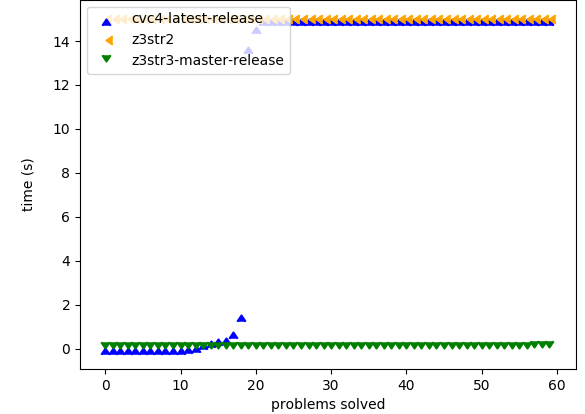
\includegraphics[width=\textwidth]{data/graphs/concats-extracts-small.png}                   
            \vspace{-0.25in}
            \caption{Performance on concats-extracts-small} 
            \label{fig:concats-extracts-small}
        \end{subfigure}
        \begin{subfigure}{.5\textwidth}
            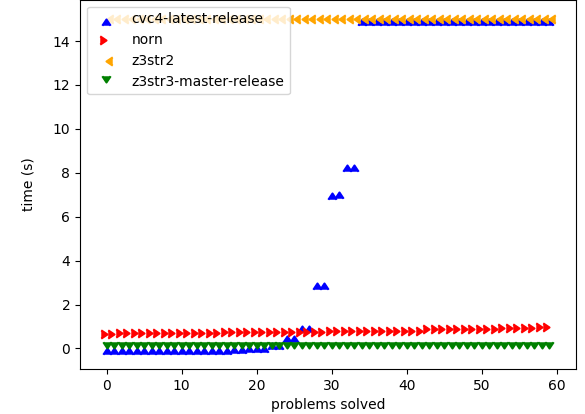
\includegraphics[width=\textwidth]{data/graphs/different-prefix.png}            
            \vspace{-0.25in}
            \caption{Performance on different-prefix}
            \label{fig:different-prefix}
        \end{subfigure}
        \vspace{-0.1in}
        \caption{Problems hard for \cvc{}}
        \label{fig:cvc-hard}
        \vspace{-0.3in}
    \end{figure}

    \begin{figure}[h]
    \vspace{-0.25in}
        \begin{subfigure}{.5\textwidth}
            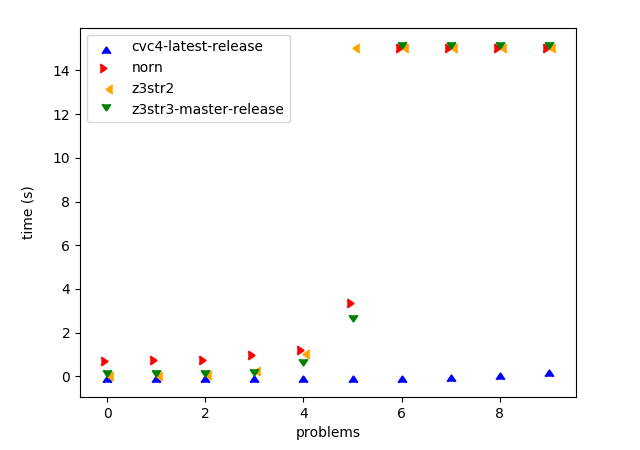
\includegraphics[width=\textwidth]{data/graphs/concats-balanced.png}
            \label{fig:concats-balanced}
            \vspace{-0.25in}
            \caption{Performance on concats-balanced}
        \end{subfigure}
        \begin{subfigure}{.5\textwidth}
            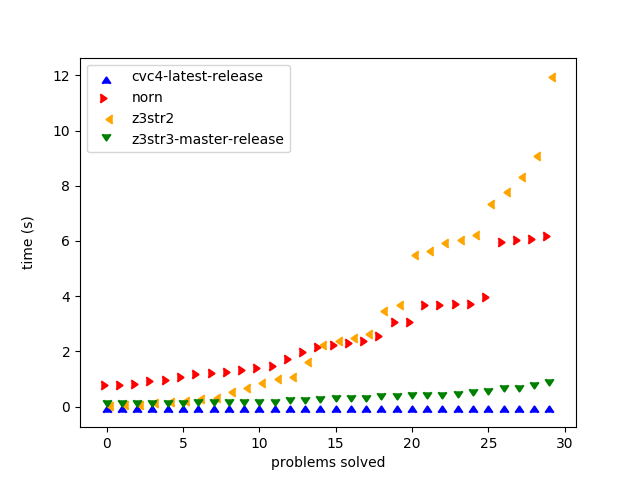
\includegraphics[width=\textwidth]{data/graphs/concats-small.png}
            \label{fig:concats-small}
            \vspace{-0.25in}
            \caption{Performance on concats-small}
        \end{subfigure}
        \vspace{-0.1in}
        \caption{Problems hard for \us{}}
        \label{fig:z3str3-hard}
        \vspace{-0.3in}
    \end{figure}

    
\section{Usefulness to \us{}: A Case Study}
\vspace{-0.1in}

        We describe the defects and missing heuristics exposed by \fuzzer{} to illustrate why \fuzzer{} is a valuable asset in solver developments.

\vspace{-0.15in}
\subsection{Defects discovered and fixed in \us{}}
\vspace{-0.1in}

The first issue we found caused \us{} to perform poorly when equivalence classes 
of arithmetic terms were very large (e.g. the lengths of many strings were equal s
to 0). This issue was detected by the \texttt{Concats} problem suite. The slowdown 
was caused by a loop over terms of such equivalence class to search for an 
integer constant. The fix was to check the root of the equivalence class for the 
integer constant, as Z3 makes "interpreted terms" (e.g. constants) the root of 
equivalence classes whenever possible. This issue was last observed in commit 
\texttt{6308636}, and was fixed in commit \texttt{3865c45}.


The second issue, which was exposed by the \texttt{Lengths} suite, caused \us{} to 
perform poorly when a variable has a large length constraint. The slowdown was 
caused by the solver performing a linear search for a satisfying length when 
producing a model for the variable. This issue was an inconsistency between the 
implementation and the behavior described in the \us{} paper \cite{z3str3}. 
This issue was last observed in commit \texttt{66bc68f}, and was fixed in commit 
\texttt{7b536e9}.    
    
    
\vspace{-0.15in}    
\subsection{Solving heuristics}
\vspace{-0.1in}

Discovering heuristics is crucial for solver efficacy improvements. Take 
conflicting constraint detection as an example. Solvers will eventually catch 
the offending terms, if they follow the string constraint solving algorithms and 
gradually propagate the (dis)equivalences discovered along the way. However, in 
many scenarios, a solver may be able to detect the conflicts before it tries to 
figure out the relationships among sub-terms and actually propagates the facts. 
The benefits are clear. It saves the efforts to reason about sub-terms and 
propagate the observations. As reported in existing works, heuristics usually 
lead to significant improvements. However, this is an extremely challenging 
process as the heuristic are usually learned from examples but it's usually hard 
to having multiple instances confirming such inefficiencies in the first place.

The instances in the \texttt{concats-big} generated by \fuzzer{} helped us 
discover a missing heuristic in \us{}. In particular, \us{} didn't make full use 
of the solving context (e.g. some terms are empty strings) to simplify the 
concatenations of a long list of string terms before trying to reason about the 
equivalences among sub-terms. It hence introduced a large number of unnecessary 
intermediate variables and fact propagations. We partially fixed this issue in 
our develop branch and observed some improvements.


% In this section, we analyse our experimental results. We discuss the causes of 
% \us{}'s poor performance on the two problem suites: \textit{concats-balanced} 
% and \textit{concats-big}. We were not equipped well enough to debug the 
% behaviours of the other solvers, but we provide our data in hopes that they will 
% be useful to the solvers' authors.

%     \subsection{\us{} on concats-balanced}
%         \todo{Dmitry with help: Explain why \us{} performs poorly on this suite.}

        
        
        
% X = "solution"
% X = (((A.B).(C.D)).((E.F).(G.H))).
%     (((I.J).(K.L)).((M.N).(O.P)))

    % \subsection{\us{} on concats-big}

    %     \todo{Dmitry with help: Explain why \us{} performs poorly on this suite.}

% X = "solution"
% X = (A.(B.(C.(D.(E.(F.(G.H)))))))
